\begin{problem}{불꽃놀이의 아름다움 2}{standard input}{standard output}{1 second}{256 megabytes}

봄 축제 때 정보과학관에서는 아무 행사도 진행되지 않는다는 것에 화가 난 민성이는 정보과학관 입구 앞에서 직접 불꽃놀이 행사를 진행하려고 한다.

정보과학관 입구 앞에 폭죽을 설치할 수 있는 $N$개의 공간과, 서로 다른 두 공간을 연결하는 도화선 $N$개가 준비되어 있다. 

$N$개의 공간은 도화선을 통해 모두 서로 연결되어 있다. 민성이는 도화선으로 직접 연결된 두 폭죽의 색이 다를 때 불꽃놀이가 아름답다고 생각한다. 하지만 불꽃놀이의 색의 종류를 늘리는 것은 비용이 많이 들기 때문에 최소한의 색을 사용하려고 한다. 아름다운 불꽃놀이를 만들기 위해 필요한 색의 개수의 최솟값을 구해보자.


\InputFile
첫째 줄에 공간의 개수 $N$이 주어진다.

둘째 줄부터 $N$개의 줄에 걸쳐 도화선이 연결하는 두 공간의 번호 $a,b$가 공백으로 구분되어 주어진다.


\OutputFile
아름다운 불꽃놀이를 만들기 위해 필요한 폭죽 색 종류의 최솟값을 출력한다.


\Examples

\begin{example}
\exmpfile{example.01}{example.01.a}%
\exmpfile{example.02}{example.02.a}%
\end{example}

\Note
제한

$3\leq N\leq 200\, 000$ 

$1\leq a,b\leq N$ 

$N$개의 공간은 도화선을 통해 서로 연결되어 있다.
도화선은 서로 다른 두 공간을 연결하며, 다른 도화선이 같은 쌍을 연결하는 경우는 없다. 

입력으로 주어지는 수는 모두 정수이다.

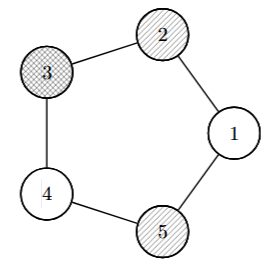
\includegraphics{5-cycle.png}

첫 번째 예시는 위 그림과 같이 3개의 색을 이용하면 아름다운 불꽃놀이를 만들 수 있고, 이보다 더 적은 색으로는 만들 수 없다.


\end{problem}

